\def\assignmenttitle{Estimating the Trajectory of a Satellite}
\def\assignmentnumber{5}
\def\assignmentdate{02-12-2011}
\def\githuburl{\small\url{https://github.com/alphabits/dtu-fall-2011/tree/master/02417/assignment-5}}
\def\githuburlfoot{\footnotesize\url{https://github.com/alphabits/dtu-fall-2011/tree/master/02417/assignment-5}}

\def\myepsilon{\varepsilon}
\def\erm{\myepsilon_{rt}}
\def\etm{\myepsilon_{\theta t}}
\def\erp{\myepsilon^p_{rt}}
\def\etp{\myepsilon^p_{\theta t}}
\def\evp{\myepsilon^p_{v_\theta t}}
\def\vecX{\myvec{X}}
\def\vecYt{\myvec{Y}_t}
\def\vece{\myvec{e}}
\def\vecSigma{\myvec{\Sigma}}
\def\vecA{\myvec{A}}
\def\vecC{\myvec{C}}


\documentclass[11pt]{article}
\linespread{1}

\renewcommand{\thefootnote}{\fnsymbol{footnote}}

\usepackage{geometry} % see geometry.pdf on how to lay out the page. There's lots.
\usepackage[utf8]{inputenc}
\usepackage[T1]{fontenc}
\usepackage{array}
\usepackage{amsmath,amssymb,latexsym,epic,eepic,epsfig,graphics,psfrag}
\usepackage{amsfonts}
\usepackage{graphicx,float}
\usepackage{color}
\definecolor{mygray}{RGB}{244,244,244}
\definecolor{gray}{gray}{0.5}
\definecolor{myredish}{RGB}{193,33,97}
\definecolor{grayblue}{RGB}{91,112,142}
\definecolor{myorange}{RGB}{255,134,0}
\definecolor{green}{rgb}{0,0.4,0}

\usepackage[english]{babel}

\usepackage[bottom]{footmisc}

\usepackage{fancyhdr}
\pagestyle{fancy}
\lhead{\small\textit{Assignment \assignmentnumber -- 02417 Time Series Analysis -- Anders Hørsted (s082382)}}
\rhead{\thepage}
\chead{}
\lfoot{}\cfoot{}\rfoot{}

\usepackage{subfigure}
\usepackage{pstricks}
\usepackage{pst-node}
\usepackage{wrapfig}
\usepackage{caption}
\usepackage{multirow}
%\usepackage{fouriernc}
%\usepackage[charter]{mathdesign}
\usepackage{lmodern}
\usepackage[normalem]{ulem}
\geometry{a4paper} % or letter or a5paper or ... etc
% \geometry{landscape} % rotated page geometry

\usepackage{url}


\makeatletter
\renewcommand*\env@matrix[1][*\c@MaxMatrixCols c]{%
  \hskip -\arraycolsep
  \let\@ifnextchar\new@ifnextchar
  \array{#1}}
\makeatother

\newcommand\myimp{\quad\Leftrightarrow\quad}
\newcommand\half{\frac{1}{2}}
\newcommand\myvec[1]{\mathbf{#1}}
\newcommand\mymod[1]{\ (\text{mod }#1)}
\newcommand\myreal{\mathbb{R}}
\newcommand\mynatural{\mathbb{N}}
\newcommand\myinteger{\mathbb{Z}}
\newcommand\mycomplex{\mathbb{C}}
\newcommand\myint{\text{int}}
\newcommand\norm[1]{||\,#1\,||}
\newcommand\bignorm[1]{\big|\big|\,#1\,\big|\big|}
\newcommand\seq[1]{\big\{#1\big\}}
\newcommand\smallseq[1]{\{#1\}}
\newcommand\smallseqtoinf[1]{\smallseq{#1}_{k=1}^\infty}
\newcommand\lonew{\ell^1_w}
\newcommand\lone{\ell^1}
\newcommand\ltwo{\ell^2(\mynatural)}
\newcommand\ip[2]{\langle#1,#2\rangle}
\newcommand\hilbert[1]{\mathcal{#1}}
\newcommand\uinf{u_{\infty}}
\newcommand\erf{\text{erf\,}}
\newcommand\infint{\int_{\infty}^{\infty}}
\newcommand\fpi{FPI}
\newcommand\E[1]{\text{E}[#1]}
\newcommand\Var[1]{\text{Var}[#1]}
\newcommand\Cov[1]{\text{Cov}[#1]}
\newcommand\myverb[1]{{\footnotesize\texttt{#1}}}
\newcommand\Yhat{\widehat{Y}}
\newcommand\given{\,|\,}

\usepackage[scaled]{beramono}
\usepackage{listings}
\lstset {                 % A rudimentary config that shows off some features.
    language=R,
    basicstyle=\scriptsize\ttfamily, % Without beramono, we'd get cmtt, the teletype font.
    commentstyle=\textit, % cmtt doesn't do italics. It might do slanted text though.
    keywordstyle=,
    identifierstyle=,
    framextopmargin=4pt,
    framexbottommargin=4pt,
    framexleftmargin=4pt,
    framexrightmargin=4pt,
    xleftmargin=4pt,
    xrightmargin=4pt,
    backgroundcolor=\color{mygray},
    frame=single,
    showstringspaces=false,
    captionpos=b,
    tabsize=4            % Or whatever you use in your editor, I suppose.
}

\renewcommand{\lstlistlistingname}{Code Listings}
\renewcommand{\lstlistingname}{Code Listing}

\usepackage{tabulary}
\newcolumntype{y}{>{\centering\arraybackslash}R}

\title{\assignmenttitle}
\date{\assignmentdate}
\author{Assignment \assignmentnumber\ -- 02417 Time Series Analysis -- Anders Hørsted (s082382)}
%\author{}
\date{} % delete this line to display the current date



%%% BEGIN DOCUMENT
\begin{document}

\maketitle

In this report the trajectory of an orbiting satellite will be reconstructed and predicted, based on 50 measurements $\{(r_t^m, \theta_t^m)\}_{t=1}^{50}$ of the position of the satellite given in polar coordinates. Due to imprecision in the measurement process, the real position of the satellite $(r_t^p, \theta_t^p)$ is related to the measurements by
\begin{align*}
    r_t^m &= r_t^p + \erm \\
    \theta_t^m &= \theta_t^p + \etm
\end{align*}
where $\erm\sim N(0,2000^2)$, $\etm\sim N(0,0.03^2)$ and $\erm$, $\etm$ are independent.

\begin{figure}[!th]
    \centering
    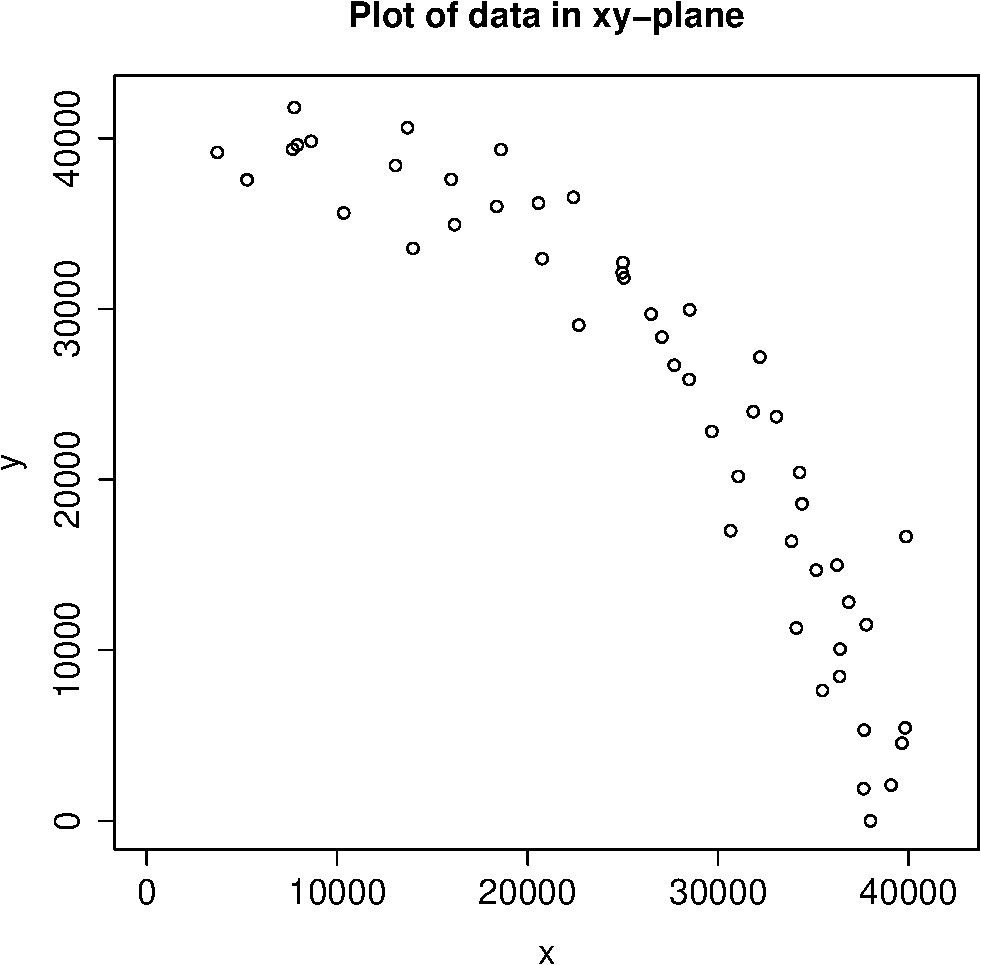
\includegraphics[width=70mm]{../plots/data.pdf}
    \caption{Plot of measured satellite position in cartesian coordinates}
    \label{fig:data}
\end{figure}

\section*{Formulating a model}
To reconstruct and predict the trajectory of the satellite, we will create a state space model. The state vector is defined as
\begin{equation*}
    \vecX_t = \begin{pmatrix}
        r^p_t \\
        \theta^p_t \\
        v^p_{\theta t}
    \end{pmatrix}
\end{equation*}
where $r^p_{t}$ is the true distance to the satellite, $\theta^p_t$ is the angle, and $v^p_{\theta t}$ is the angle velocity. It is assumed that the trajectory is well approximated by a circle, but to include deviations from a perfect circle, we define the random deviations
\begin{equation*}
    \erp \sim N(0,500^2), \quad \etp\sim N(0,0.005^2), \quad \evp \sim N(0, 0.005^2)
\end{equation*}
and then model the dynamics of the state vector by the equations
\begin{align*}
    r^p_t &= r^p_{t-1} + \erp \\
    \theta^p_t &= \theta^p_{t-1} + v^p_{t-1} + \etp \\
    v^p_t &= v^p_{t-1} + \evp
\end{align*}
From these equation it is seen, that we model the radius and angle-velocity to be constant, as they would be for prefect uniform circular motion.
To write the state space model on matrix form, we define the measurement vector by
\begin{equation*}
    \vecYt = \begin{pmatrix}
        r^m_t \\
        \theta^m_t
    \end{pmatrix}
\end{equation*}
and two random vectors by
\begin{equation*}
    \vece_1 = \begin{pmatrix}
        \erp \\
        \etp \\
        \evp
    \end{pmatrix}, \quad \vece_2 = \begin{pmatrix}
        \erm \\
        \etm
    \end{pmatrix}
\end{equation*}
Since $\erp,\etp$ and $\evp$ are independent the covariance between any two of them is 0. $\erm$ and $\etm$ are also independent and therefore the covariance between them is also 0. We then get
\begin{equation*}
    \vecSigma_1 = \Var{\vece_1} = \begin{bmatrix}
        500^2 & 0 & 0 \\
        0 & 0.005^2 & 0 \\
        0 & 0 & 0.005^2
    \end{bmatrix}, \quad \vecSigma_2 = \Var{\vece_2} = \begin{bmatrix}
        2000^2 & 0 \\
        0 & 0.03^2
    \end{bmatrix}
\end{equation*}
By setting
\begin{equation*}
    \vecA = \begin{bmatrix}
        1 & 0 & 0 \\
        0 & 1 & 1 \\
        0 & 0 & 1
    \end{bmatrix}, \quad \vecC = \begin{bmatrix}
        1 & 0 & 0 \\
        0 & 1 & 0
    \end{bmatrix}
\end{equation*}
the state space model can now be expressed by the system equation
\begin{equation*}
    \vecX_t = \vecA\vecX_{t-1} + \vece_1
\end{equation*}
and the observation equation
\begin{equation*}
    \vecYt = \vecC\vecX_t + \vece_2
\end{equation*}

Using the defined model the trajectory can now be reconstructed and predicted by using the Kalman filter. To actually use the Kalman filter, it needs to be implemented.

\section*{Implementing the Kalman filter}
The implementation of the Kalman filter is shown in listing~\ref{lst:kalman}. It is a function that takes the model defining parameters \myverb{A,B,C,u,S.1} and \myverb{S.2}, the initialization parameters \myverb{mu0} and \myverb{V0}, and the observations \myverb{Y}. The code is more or less self explaining and is based on equation 10.73-10.80 in \cite{hm}. The function returns a list with the reconstructed state vector for each iteration, the final covariance matrix for the one-step prediction of the state vector, the Kalman Gain from each iteration and the final one-step prediction of the state vector. 

\vspace{3mm}
\lstinputlisting[caption={Implementation of the Kalman filter},label=lst:kalman]{../src/kalmanfilter.R}


\section*{Reconstructing the trajectory}
In this section the implementation of the Kalman filter is used to reconstruct the trajectory of the satellite. To run the Kalman filter the initial parameters $\myvec{\mu}_0$ and $\myvec{V}_0$ needs to be defined. As long as there are many observations, the result isn't very sensitive to the initial conditions. We set
\begin{equation*}
    \myvec{\mu}_0 = \begin{pmatrix}
        r^m_1 \\
        \theta^m_1 \\
        0
    \end{pmatrix}, \quad \myvec{V}_0 = \begin{bmatrix}
        0, 0, 0 \\
        0, 0, 0 \\
        0, 0, 0
    \end{bmatrix}
\end{equation*}
and then run the Kalman implementation from the previous section\footnote{See \appref{runkalman} for the actual code that runs the Kalman filter}. Since the implementation returns the reconstructed state vector for each iteration, the reconstructed trajectory can easily be plotted\footnote{See \appref{reconstruct} for the code} as shown in figure~\ref{fig:reconstruction}

\begin{figure}[ht]
    \centering
    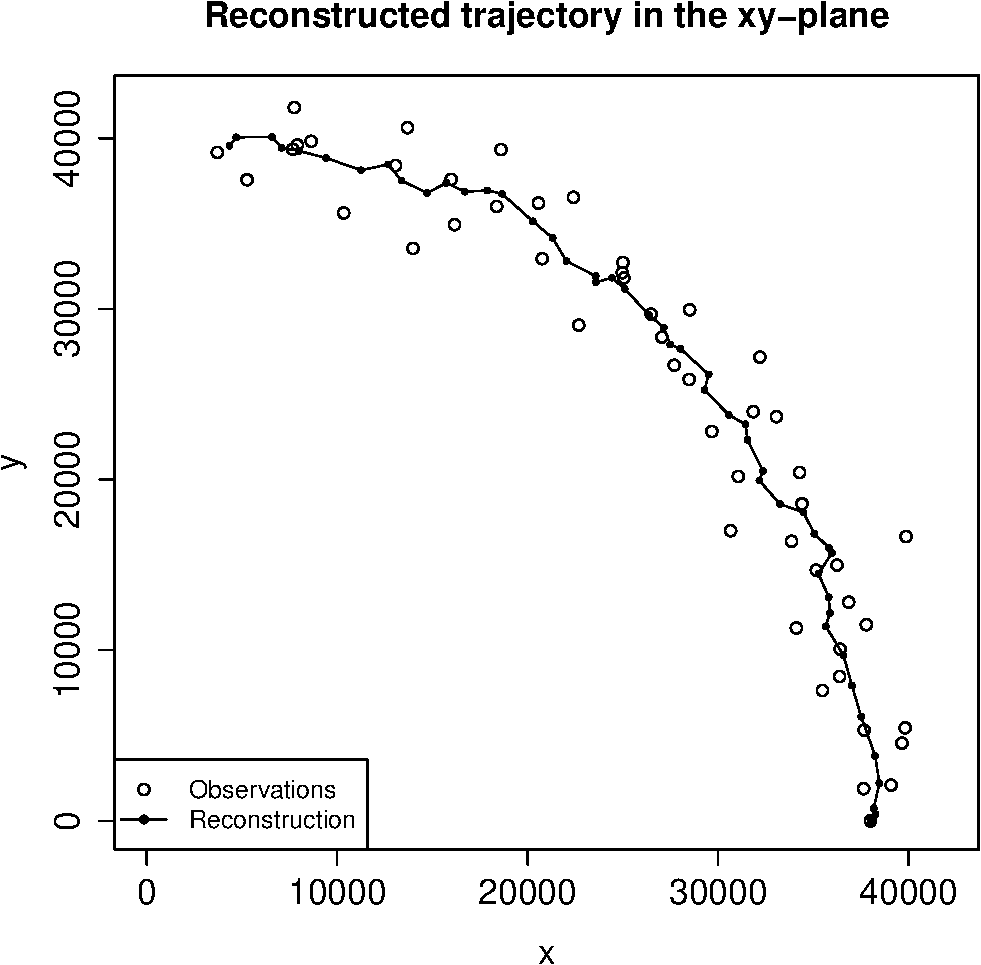
\includegraphics[width=70mm]{../plots/reconstruction.pdf}
    \caption{The reconstructed trajectory calculated with the Kalman filter}
    \label{fig:reconstruction}
\end{figure}

It is seen that the Kalman filter is pretty robust even when the data contains large errors. From the output of the Kalman filter function it is seen that the Kalman Gain converges to a constant value after about 30 iterations which is expected.


\section*{Predicting the trajectory}
The satellite position for the 6 next time steps should now be predicted. The Kalman filter only gives one-step predictions, but using the equations
\begin{align}
    \widehat{\myvec{X}}_{t+k+1|t} &= \myvec{A}\widehat{\myvec{X}}_{t+k|t} + \myvec{B}\myvec{u}_{t+k} \label{eq:ksteppred}\\
    \myvec{\Sigma}^{xx}_{t+k+1|t} &= \myvec{A}\myvec{\Sigma}^{xx}_{t+k|t}\myvec{A}^T + \myvec{\Sigma}_1 \label{eq:kstepcovar}
\end{align}
the predictions for later steps can also be found. From the equations and the definition of $\myvec{A}$ it is clear that the prediction of $r^p_{t+k}$ is constant for any $k>0$. To get all predictions of $r^p_{t+k}$ and $\theta^p_{t+k}$ the Kalman filter is first run on the data. The output from the Kalman filter gives the 1-step prediction, and then iterating equation (\ref{eq:ksteppred}) and (\ref{eq:kstepcovar}) 5 times gives the $2,3\dots,6$-step predictions. The results are shown in table~\ref{tbl:predictions}

\begin{table}
    \centering
    \begin{tabular}{lccc}
        $k$ & $\widehat{r}_{50+k|50}$ & $1.96\sigma_{\hat{r}}$ & 95\% CI \\\hline
        1 & 39805.96 & 2086.07 & [37719.89; 41892.03] \\
2 & 39805.96 & 2304.80 & [37501.16; 42110.76] \\
3 & 39805.96 & 2504.50 & [37301.47; 42310.46] \\
4 & 39805.96 & 2689.40 & [37116.56; 42495.37] \\
5 & 39805.96 & 2862.39 & [36943.57; 42668.35] \\
6 & 39805.96 & 3025.51 & [36780.45; 42831.47] 
\\\hline
    \end{tabular}
    \hspace{0.5mm}
    \begin{tabular}{lccc}
        $k$ & $\widehat{\theta}_{50+k|50}$ & $1.96\sigma_{\hat{\theta}}$ & 95\% CI \\\hline
        1 & 1.49 & 0.05 & [1.43; 1.54] \\
2 & 1.51 & 0.07 & [1.44; 1.58] \\
3 & 1.54 & 0.09 & [1.45; 1.63] \\
4 & 1.56 & 0.11 & [1.45; 1.67] \\
5 & 1.59 & 0.13 & [1.45; 1.72] \\
6 & 1.61 & 0.16 & [1.46; 1.77] 
\\\hline
    \end{tabular}
    \caption{Prediction and confidence intervals for $\widehat{r}$ and $\widehat{\theta}$}
    \label{tbl:predictions}
\end{table}

To visualize the predictions a plot is made and shown in figure~\ref{fig:all-predictions}. From the figure it is seen (confirmed, since we already knew it) how the predictions lie equally spaced on a perfect circle. This is probably not how the actual position is going to end up, so we would like to give an idea of the uncertainty of the predictions.

\begin{figure}[!ht]
    \centering
    \mbox{\subfigure{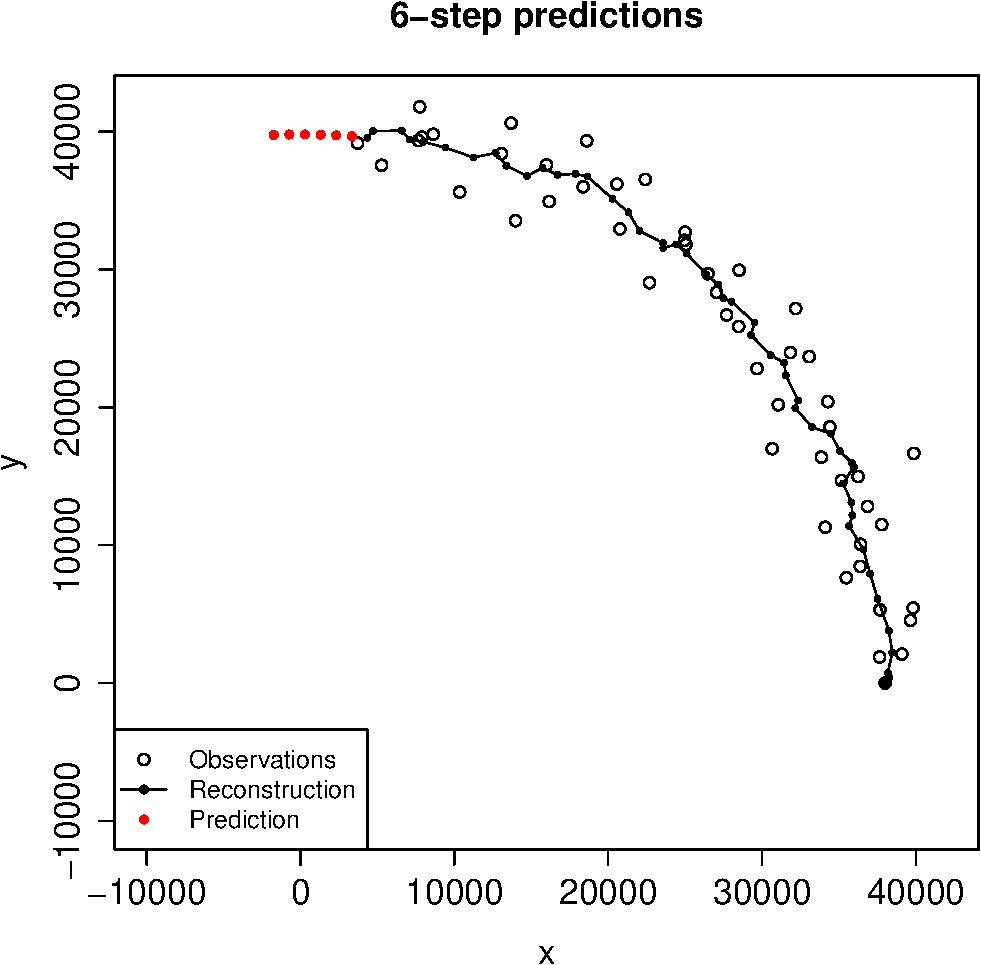
\includegraphics[width=70mm]{../plots/all-predictions.pdf}} \quad 
            \subfigure{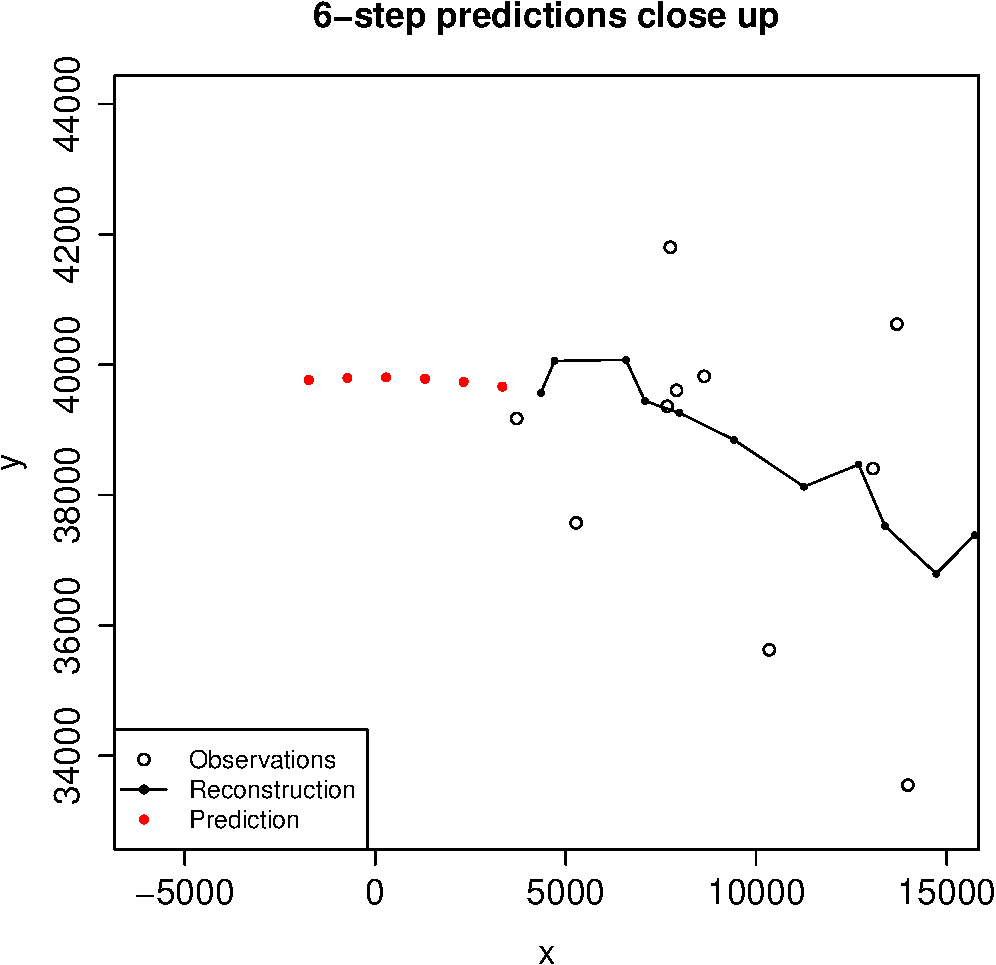
\includegraphics[width=70mm]{../plots/all-predictions-magnified.pdf}}}
    \caption{Predictions of the satellite position 6 step ahead}
    \label{fig:all-predictions}
\end{figure}

The uncertainty is already given in table~\ref{tbl:predictions}, but to give an better idea the 6 predictions are plotted on separate plots including their respective confidence intervals. The plots are shown in figure~\ref{fig:predictions-with-conf-1} and figure~\ref{fig:predictions-with-conf-2} and it is seen how the uncertainty grows larger for each time step away from the time of prediction. This was expected both intuitively and from equation (\ref{eq:kstepcovar}), but it is still worth noticing that the right side of the 6-step prediction confidence interval is almost identical to the right side of the 1-step prediction confidence interval. With a 95\% confidence, we can't reject the possibility that the satellite will be in the same spot 1 and 6 time steps ahead. Still the theory tells us that these are the best prediction we can give, as long as we don't get any new observations.

\begin{figure}[!hb]
    \centering
    \mbox{\subfigure{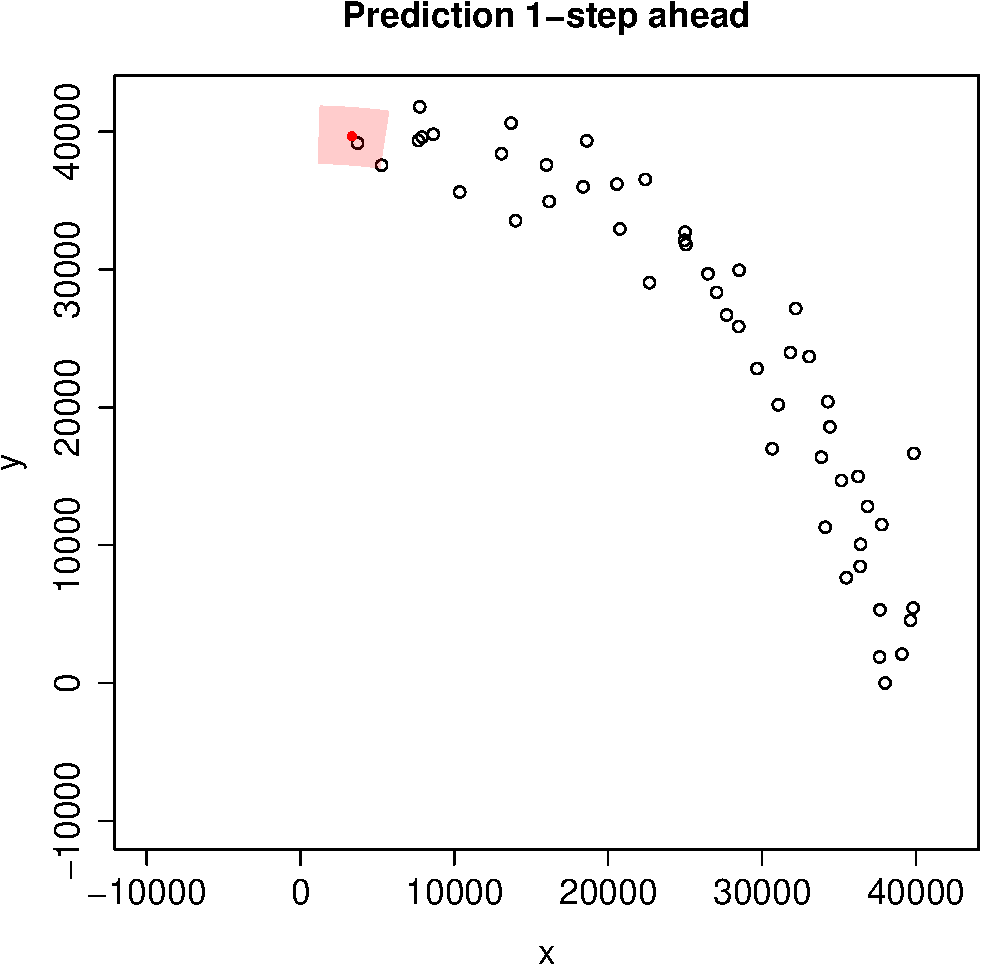
\includegraphics[width=70mm]{../plots/prediction-1.pdf}} \quad 
            \subfigure{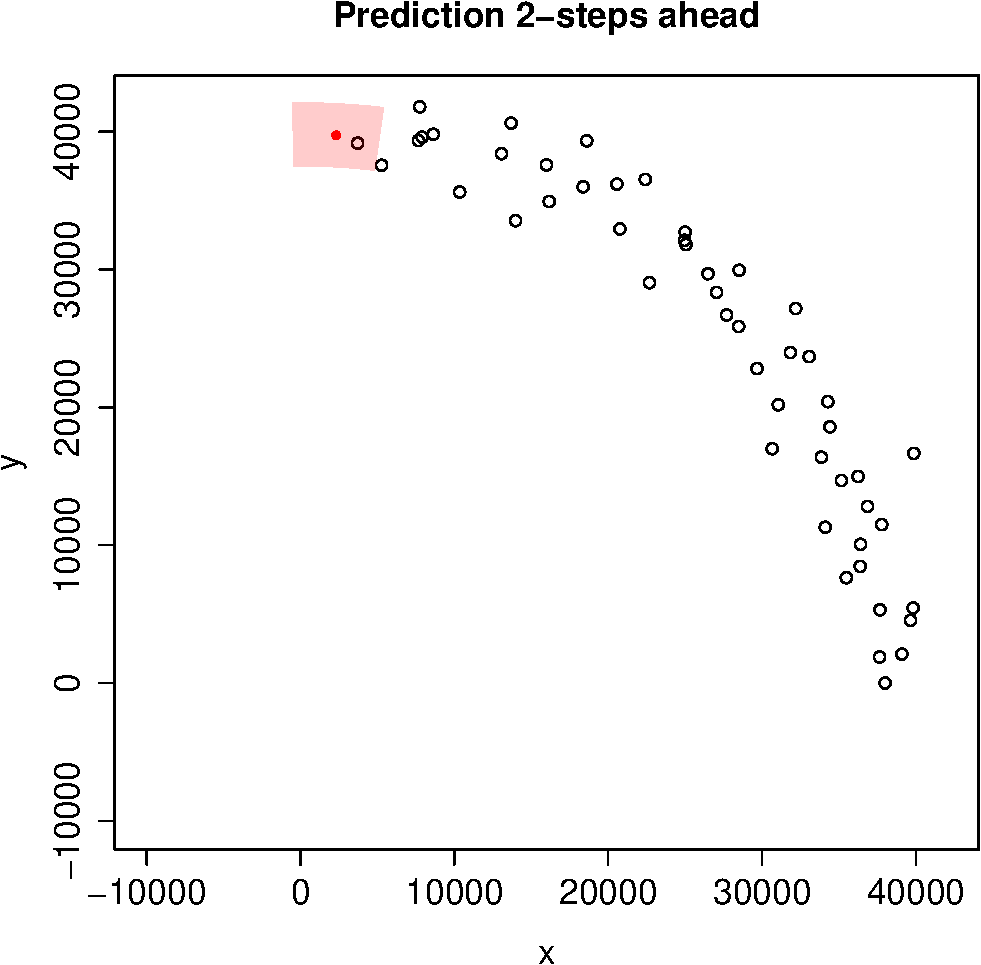
\includegraphics[width=70mm]{../plots/prediction-2.pdf}}}
    \mbox{\subfigure{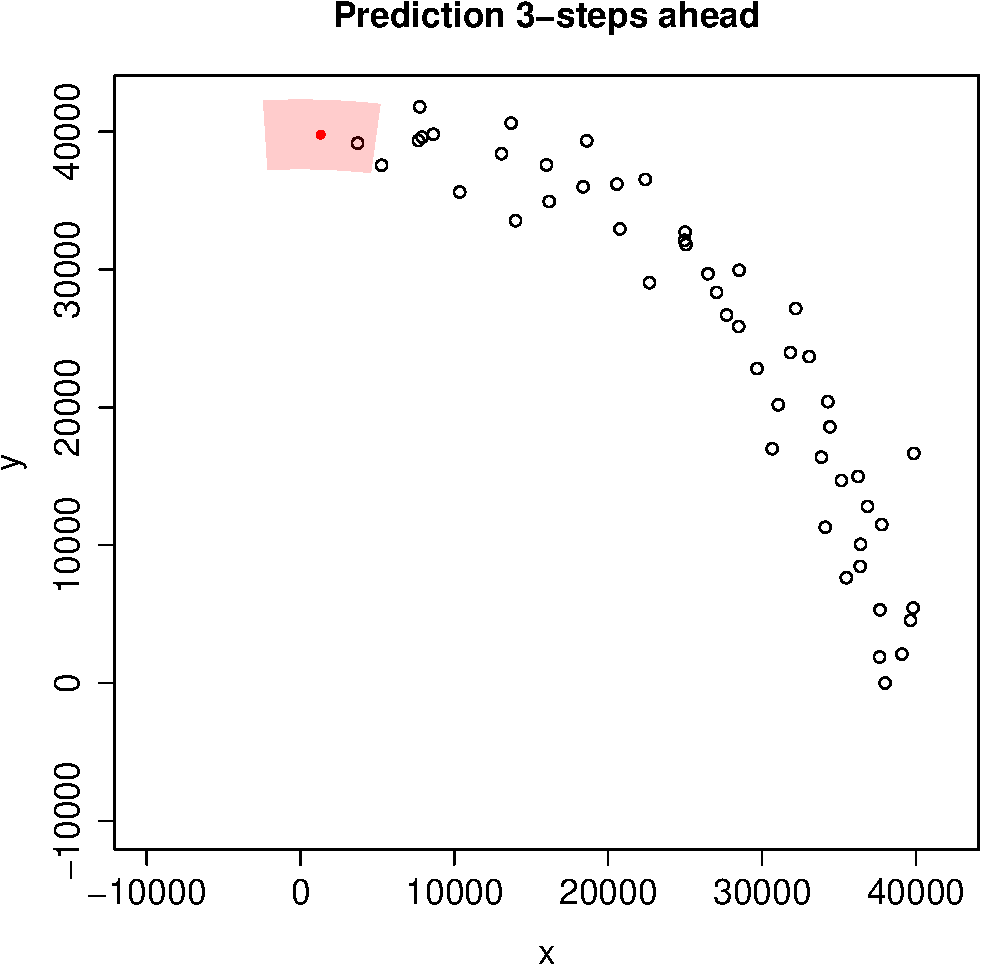
\includegraphics[width=70mm]{../plots/prediction-3.pdf}} \quad 
            \subfigure{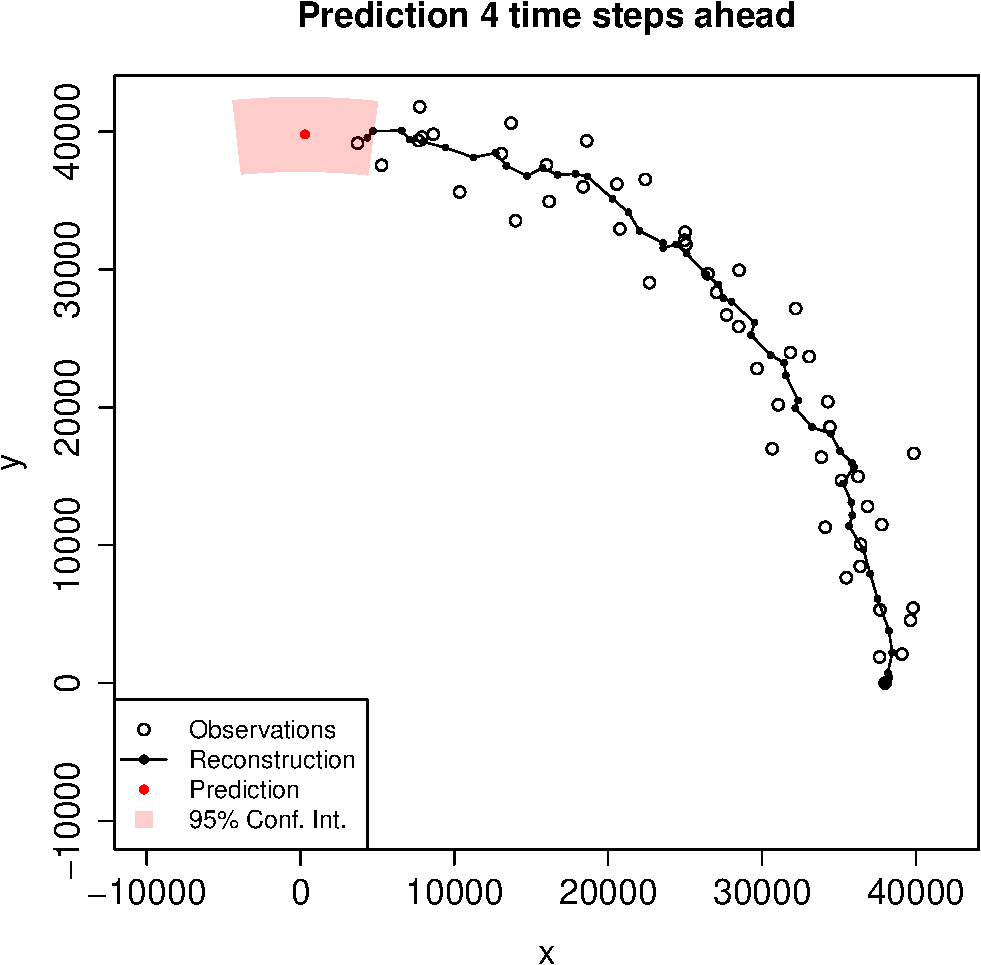
\includegraphics[width=70mm]{../plots/prediction-4.pdf}}}
    \caption{Plots of the 1-,2-,3-, and 4-step predictions including confidence intervals. 5- and 6-step are on the next page.}
    \label{fig:predictions-with-conf-1}
\end{figure}

\begin{figure}
    \centering
    \mbox{\subfigure{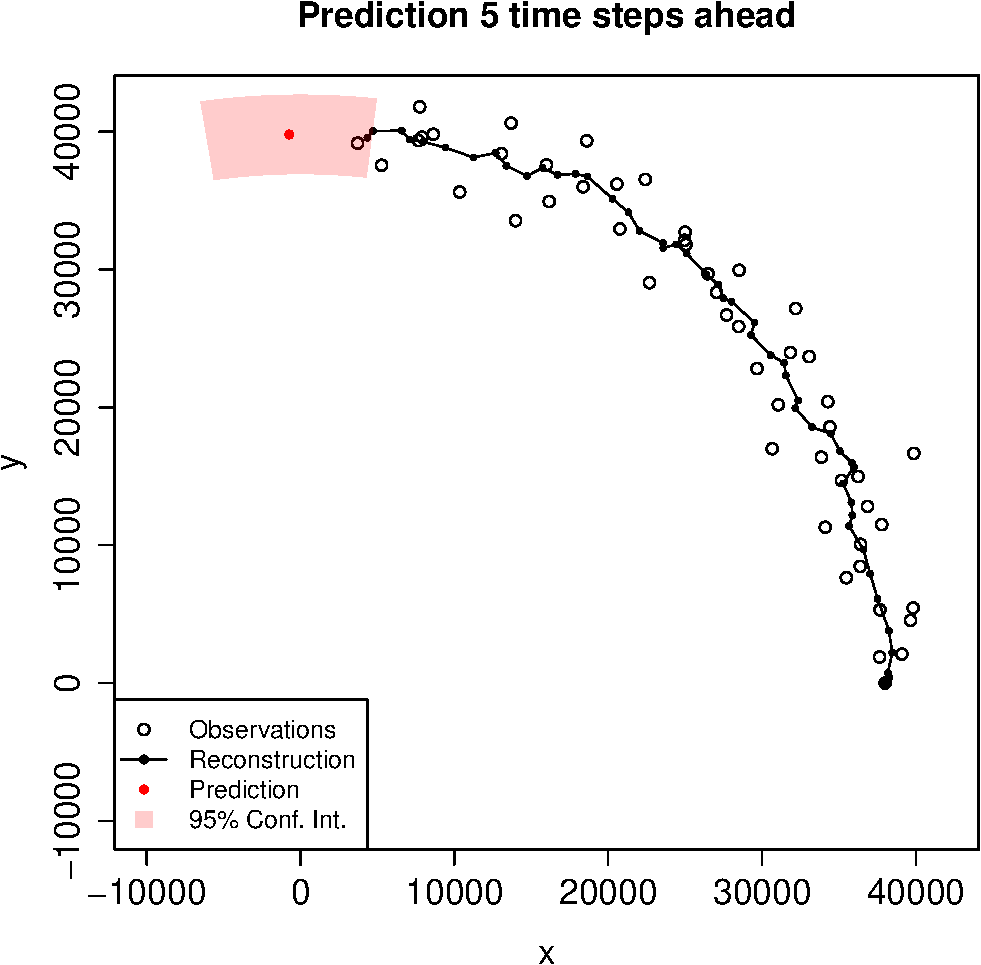
\includegraphics[width=70mm]{../plots/prediction-5.pdf}} \quad 
            \subfigure{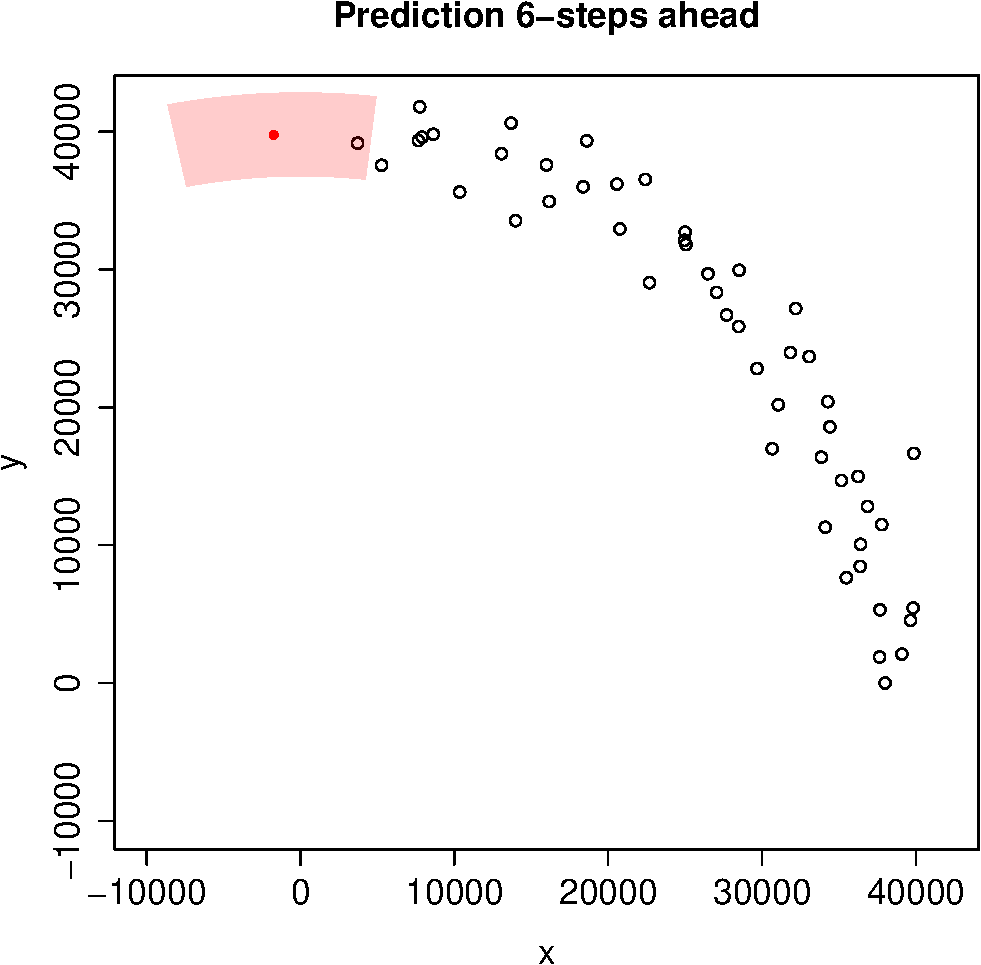
\includegraphics[width=70mm]{../plots/prediction-6.pdf}}}
    \caption{Plots of the 5-, and 6-step predictions including confidence intervals}
    \label{fig:predictions-with-conf-2}
\end{figure}

\FloatBarrier

\pagebreak

\renewcommand\thesection{\Alph{section}}
\section{Appendices}

All R code used for this assignment is included here. All source code incl.
latex code for this report can be found at \githuburl

\subsection{Load data script}
\lstinputlisting{../src/loaddata.R}

\subsection{Helper functions}
\lstinputlisting{../src/functions.R}

\subsection{Plot data script}
\lstinputlisting{../src/plotdata.R}

\subsection{Running the Kalman filter}\label{app:runkalman}
\lstinputlisting{../src/runkalman.R}

\subsection{Plot reconstructed trajectory}\label{app:reconstruct}
\lstinputlisting{../src/reconstruction.R}

\subsection{Predicting trajectory}\label{app:predict}
\lstinputlisting{../src/predict.R}

\pagebreak

\begin{thebibliography}{9}

\bibitem{hm}
  Henrik Madsen,
  \emph{Time Series Analysis}.
  Chapman \& Hall/CRC,
  1st Edition,
  2008.

%\bibitem{taleb}
%  Nassim Nicholas Taleb,
%  \emph{The Black Swan}.
%  Random House Trade Paperbacks
%  2nd Edition,
%  2010.

\end{thebibliography}


\end{document}
